%
% Frameworks / Bibliotheken
%
\chapter{\label{chap:state}Bestehende offlinefähige Technologien}
Um eine Webapplikation offlinefähig zu machen, müssen alle Daten auf dem Client gespeichert werden und von diesem zu jeder Zeit abrufbar sein.
Für Anwendungen mit einer serverseitigen Datenbank ist die Synchronisation der Daten zwischen Server und Client notwendig.\\
Es gibt verschiedene Technologien, die sich diesen Problematiken widmen.
Diese umfassen Bibliotheken und Frameworks, die die Entwicklung offlinefähiger Anwendungen unterstützen, sowie Datenbanklösungen. In den nächsten Punkten werden einige dieser Technologien näher beschreiben.
%
% webpack offline-plugin
%
\section{Offline plugin für webpack}
Webpack ist ein JavaScript `Bundler` und bündelt alle Skripte, Bilder und \gls{Assets} für die Verwendung in Browsern.\\
Das Offline Plugin bietet Offlinefunktionalität für Webpackprojekte indem es die gebündelten, also von Webpack generierten \gls{Assets} cached.
Dazu benutzt es intern den ServiceWorker und AppCache als Reserve, für den Fall dass der Browser ServiceWorker nicht unterstützt~\cite{webpack-gh}.\\
Auch ungebundelte \gls{Assets} können über das Plugin gecached werden. Diese Dateien müssen dann in den Optionen explizit angegeben werden. Auch der ServiceWorker und der AppCache lassen sich über die Optionen konfigurieren oder auch ausschalten~\cite{webpack-opt}.\\
Es werden allerdings nur die \gls{Assets} und nicht die von BenutzerInnen generierten Daten gecached. Diese müssen manuell im gespeichert werden.
%
% redux-offline
%
\section{\label{sub:reduxoffline}Redux Offline}
%``Persistenter Redux store für \it{reasonaboutable}\tm ~Offline-First Anwendungen``. \\
Redux Offline kann nur zusammen mit Redux verwendet werden~\cite{redux-req}. Deswegen ist für die Verwendung von Redux Offline die Implementierung von Redux vorausgesetzt.
%
% Redux
%
% Alles beginnt mit dem Aufruf von \tt{store.dispatch(action)} von jeder beliebigen Stelle in der Anwendung. Die Aktion die beschreibt was passiert heißt \tt{toggleEdit} und sieht im Beispiel des Ansichtswechsels aus wie in Zeile drei bis fünf.\\
% Der \tt{Store} ruft nun den \tt{Reducer} auf
\sub{Redux}
Redux ist eine JavaScript Bibliothek die Probleme im Zusammenhang mit dem \it{Zustand} einer Anwendung löst.
Redux ist eine Bibliothek zur Zustandsverwaltung in JavaScriptanwendungen.
Es gibt einen zentralen Ort, in dem der \it{Zustand} der App gespeichert ist, auf den von jeder Komponente aus zugegriffen werden kann.
Dieser Ort wird \sc{Store} genannt und jede Applikation hat genau einen davon. 
Als einzige Informationsquelle für den Store als zentralen Speicher dienen Aktionen. 
Sie senden Daten von der Anwendung mittels \tt{store.dispatch()} an den \sc{store} und beschreiben dabei nicht wie etwas passiert, sondern was passiert.
Der dritte wichtige Bestandteil von Redux sind die \sc{Reducer}. Sie spezifizieren wie der Status sich als Reaktion auf die Aktionen ändert~\cite{redux}.\\
Der Datenfluss in der Reduxarchitektur ist unidirektional. Zur Veranschaulichung wird anhand der folgenden Abbildung der Redux Datenfluss beschrieben.
%
\begin{figure}[H]
  \centering
  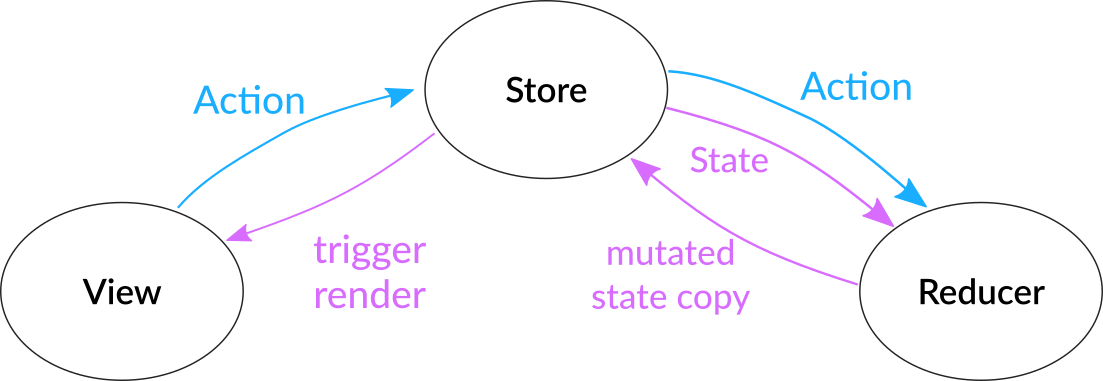
\includegraphics[width=0.8\textwidth]{redux-flow}
  \grayRule
  \caption{Redux Datenfluss}
  \label{fig:rdx-dataflow}
\end{figure}
% 
Zuerst sendet die View eine Aktion an den Store. Dieser empfängt die Aktion und schickt sie zusammen mit dem Applikationsstatus an den \sc{Reducer}.
Der \sc{Reducer} erstellt eine Kopie des Status, verändert diese und schickt sie wieder zurück an den \sc{Store}. Der \sc{Store} ersetzt nun den alten mit dem neuen Status und löst ein erneutes Rendern der View aus.
% 
% Redux Offline
% 
\sub{Redux Offline}
Redux Offline erweitert Redux um einen persistenten \sc{Store} mit Offline-First Technologie und  ist kompatibel mit allen *View Frameworks wie React\footnote{JavaScript Bibliothek: \url{https://reactjs.org/}}, Vue\footnote{JavaScript Framework: \url{https://vuejs.org/}}, oder Angular\footnote{JavaScript Framework: \url{https://www.angular.io}}~\cite{redux-offline-compabilaty}.
Es umfasst unter Anderem netzwerkfähige \gls{API}-Aufrufe, das Persistieren des Zustands der Anwendung, das speichern von Aktionen, die Behandlung von Fehlern und erneute Versuche die Verbindung wieder herzustellen.
Redux Offline verspricht nicht, die Webanwendung komplett offlinefähig zu machen. Um \gls{Assets} zwischenzuspeichern, muss zusätzlich noch ein ServiceWorker implementiert sein ~\cite{redux-offline-gh}.\\
Die Idee hinter Redux Offline ist, dass der Redux \sc{Store} die Datenbank ersetzt~\cite{redux-offline}. Bei jeder Änderung wird der Redux \sc{Store} auf dem Datenträger gespeichert, und bei jedem Start automatisch neugeladen. Für das Speichern der Daten in einer lokalen Datenbank wird intern \hyperref[sub:reduxpersist]{Redux Persist} verwendet.\\\\
Eine mit Redux Offline erstellte Anwendung funktioniert ohne weitere Codeimplementierung offline im Lesemodus, da das Lesen und Schreiben aus der lokalen Datenbank bereits eigebunden ist.
Damit die Anwendung auch im Schreibmodus offline funktioniert, müssen einige Anpassungen vorgenommen werden.
Sämtliche Daten der Anwendung können nur über Aktionen manipuliert werden. 
Alle netzwerkgebundenen Aktionen werden  in einem \sc{store}internem \gls{Queue} gespeichert und müssen mit einem Metaattribut dekoriert werden um offline arbeiten zu können. Durch die Metaattribute weiß die Anwendung was vor der eigentlichen Ausführung der Aktion und was danach zu tun ist. 
Es gibt drei Metadaten die Redux Offline interpretieren kann:\\
\tt{meta.offline.effect} - Die initiale Aktion wird ausgeführt. Hier kann eine URL angegeben werden die Redux Offline anfragen soll.\\
\tt{meta.offline.commit} - Hier wird die Aktion definiert die ausgeführt wird sobald die Netzwerkanfrage erfolgreich ist.\\
\tt{meta.offline.rollback} - Hier kann die Aktion angegeben werden, die bei  permanent fehlgeschlagener Internetverbindung oder wenn der Server einen Serverfehler zurückgibt gefeuert wird.
Dann fügt Redux Offline dem \sc{Appstate} automatisch ein \tt{offline} Objekt hinzu. Dort wird unter anderem ein Array namens \tt{outbox} verwaltet wird.
Dieses Array repräsentiert den \gls{Queue}. Hier werden die Aktionen inklusive Metadaten gespeichert, um bei bestehender Internetverbindung abgearbeitet zu werden~\cite{redux-offline-docs}.
Die von Jani Eväkallio erstellte Grafik \ref{fig:redux-offline} veranschaulicht die oben erklärte Architektur.\\
%
\begin{figure}[h]
  \centering
  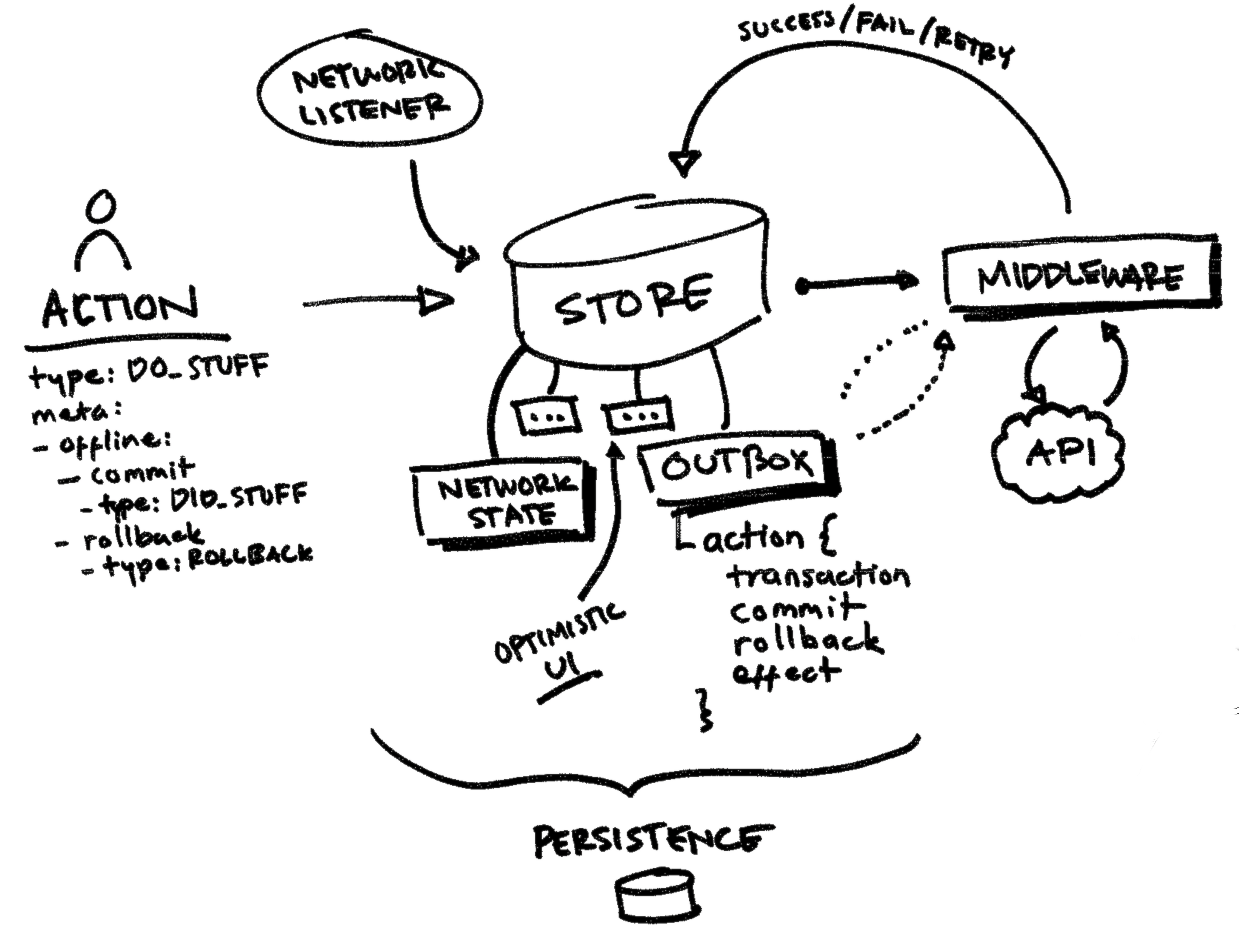
\includegraphics[width=0.8\textwidth]{redux-offline-new}
  \grayRule
  \caption[Redux Offline]{Redux Offline Architektur~Quelle:~\cite{redux-offline}}
  \label{fig:redux-offline}
\end{figure}
%
Links ist eine Aktion zu sehen die Zeug machen möchte. Sie hat ein Mateattribut das weitere Aktionen definiert. Eine Aktion für den Erfolg und eine für den Fehlschlag von `DO\_STUFF`.
In der Mitte ist der \sc{Store} zu sehen. Der \sc{Store} kennt den Netzwerkstatus und hat den \gls{Queue} namens \tt{outbox} in dem Aktionen mitsamt ihrer Metafelder gespeichert werden. Rechts befindet sich das \gls{API}, das über die \gls{Middleware} mit dem \sc{Store} redet.\\
Wird die Aktion 'DO\_STUFF' gefeuert gelangt sie in den \sc{Store}, damit dieser den \sc{AppState} aktualisieren kann, und wird ersteinmal im \gls{Queue} gespeichert. Ist die Anwendung online, wird sie sofort abgearbeitet. Wenn nicht wird sie dort gespeichert bis die Anwendung wieder eine Verbindung zum Internet hat.   
% \subsub{Konflikte}
%
% redux persist
%
\sub{\label{sub:reduxpersist}Redux Persist}
Redux Persist ist eine Bibliothek, die als Wrapper für den Redux Store funktioniert. Mit Redux Persist wird der \tt{state} automatisch lokal, per default im LocalStorage, gespeichert~\cite{redux-persist}.
Es kann konfiguriert werden wo die Daten gespeichert werden. Hier gibt es diverse Möglichkeiten wie zum Beispiel im SessionStorage, per localForage oder in Dateisystemen~{redux-persist-gh}. LocalForage ist eine Bibliothek mit der Daten in IndexedDB, WebSQL gespeichert werden können. Wenn der Browser die Speichermöglichkeiten nicht unterstützt, wird der LocalStorage genommen~\cite{localforage}.\\
Es ist auch möglich einen eigenen Speicher zu konfigurieren. Die einzige Voraussetzung hierfür ist, das \gls{API} muss die Standardmethoden \tt{setItem}, \tt{getitem} und \tt{removeItem} implementieren und Promises unterstützen~\cite{redux-persist-gh}.
%
% redux optimist
%
% \sub{redux-optimist}
%
% react-native-offline
%
\sub{react-native-offline}
React Native = JavaScript React Framework um native, mobile Apps zu bauen. blabla\\
Behandelt online/offline Verbindung. Kann die Internetverbindung auch regelmäßig prüfen\\
Speichert nur den Status online/offline im store. -> erlaubt so unterschiedliches Rendern von Componenten.\\

\tt{const YourComponent = ({ isConnected }) => (\\
  <Text>{isConnected ? 'I am connected to the internet!' : 'Offline :('}</Text>\\
  );\\}\\
  Zusammen mir Redux hat es einen `Mehrwert`:
  Hat dann einen `Offline-\gls{Queue} um Aktionen zu wiederholen (im Intervall) \tt{meta.retry? \textcolor{gray}  {Array of actions which, once dispatched, will trigger a dismissal from the queue}} ~ oder nicht \tt{meta.dismiss? []}.\cite{rn-offline-gh}
  % \cite{rn-offline-medium}

%
% hoodie
%
\section{hoodie}
HOODIE ist eine JavaScript Bibliothek für offlinefähige Webapplikationen, die ein komplettes Backend zur Verfügung stellt. Wird HOODIE für die Entwicklung einer Webanwendung verwendet, muss also lediglich das Frontend implementiert werden. Den Rest erledigt die Bibliothek. Über eine integrierte Programmierschnittstelle kommuniziert die Anwendung mit dem von HOODIE zur Verfügung gestelltem Backend. Über das \gls{API} können unter Anderen BenutzerInnen authentifiziert, Daten gespeichert und synchronisiert werden~\cite{hoodie}.\\
Anhand der Abbildung \ref{fig:hoodie} wird erklärt wie HOODIE funktioniert.
\begin{figure}[H]
  \centering
  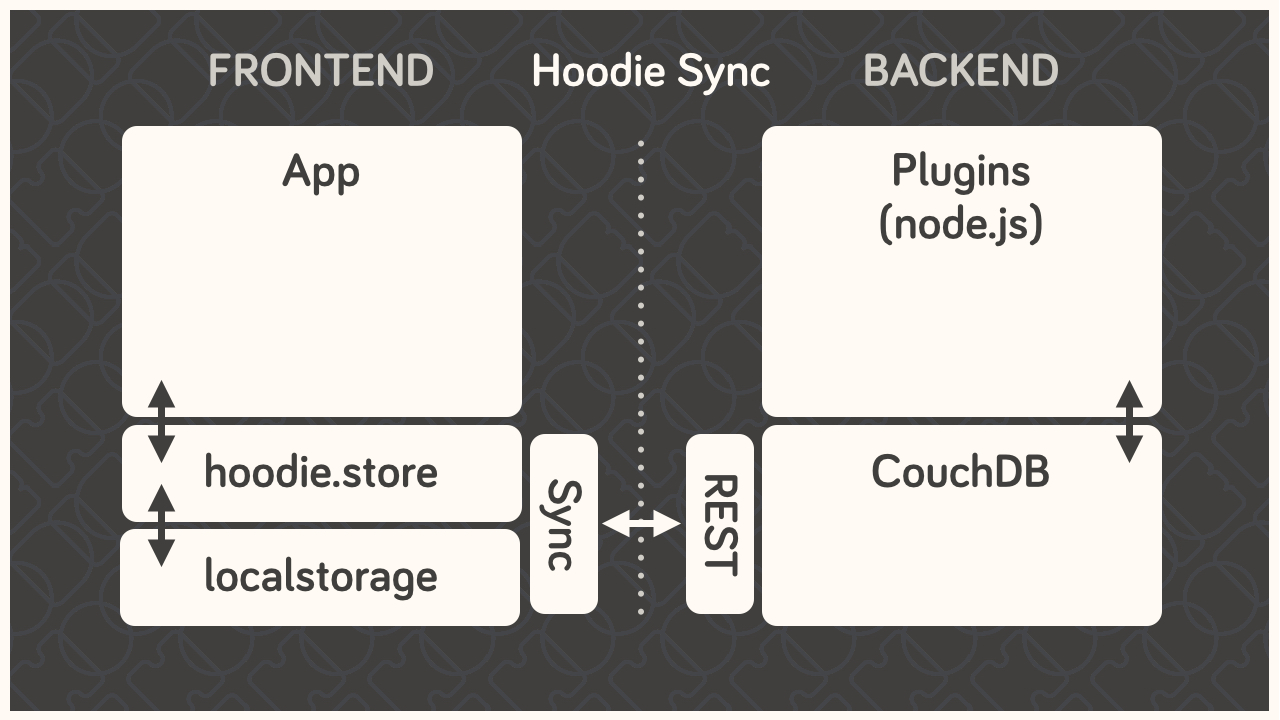
\includegraphics[width=0.8\textwidth]{hoodie}
  \grayRule
  \caption[HOODIE Architektur]{HOODIE Architektur~Quelle:~\cite{hoodie-how}}
  \label{fig:hoodie}
\end{figure}
Im Frontend--Bereicht ist die App zu sehen die über das HOODIE \gls{API} mit dem lokalen Speicher kommuniziert. Die Anwendung spricht niemals direkt mit dem Server oder der Datenbank. Für die lokale Speicherung der Daten benutzt HOODIE intern PouchDB, was wiederum IndexedDB verwendet. Durch das lokale Speichern sind die Daten auch offline verfügbar. Dann werden über eine \gls{REST} Schnittstelle mit einer CouchDB synchronisiert. CouchDB ist eine Datenbank mit der Superkraft des Synchronisierens und in HOODIE haben alle AnwenderInnen ihre eigene private CouchDB. Hinter der Datenbank befindet sich ein kleiner Server der auf die Daten in der CouchDB reagiert, die wiederum die Änderungen an den Client schickt ~\cite{hoodie-how}.
So können NutzerInnen nur auf ihre eigenen Daten zugreifen. Wenn es mehrere Geräte gibt, die mit einem Account assoziiert werden, werden die Änderungen von einem Gerät zuerst auf die serverseitige CouchDB synchronisiert, um dann von dort in die lokalen Datenbanken der anderen Geräte zu gelangen.\\
Dadurch, dass das Frontend und das Backend nicht direkt miteinander sprechen, ist die Funktionalität beider Komponenten auch dann gewährleistet, wenn die Verbindung unterbrochen wird.
%
% realm
%
\section{\label{sub:realm}Realm}
Realm ist eine Backendtechnologie für mobile Anwendungen und umfasst die Realm--Datenbank und den Realm Object--Server.
Die Datenbank ist quelloffen, der Object--Server jedoch nicht -- dieser ist außerdem nicht kostenfrei~\cite{realm}.\\
Die Realm--Datenbank ist eine objektorientierte, plattformübergreifende lokale Datenbank die eine Echtzeitsynchronisation mit dem Realm Object--Server bereitstellt.
Der Object--Server fungiert als \gls{Middleware}-Komponente in der mobilen \gls{App} und handhabt unter anderem die Ereignisbehandlung und Datensynchronisation.
Im Zusammenspiel ermöglichen die beiden Technologien die Erstellung von offlinefähigen, kollaborativen, mobilen Anwendungen~\cite{realm_whitepaper}.\\\\
%
%
Zur Offline First--Funktionalität stellt Realm eine umfassende Lösung bereit.
Die lokale Realm--Datenbank unterstützt die Echtzeitsynchronisation von Daten, sodass alle Änderungen sofort automatisch gesendet werden.
Das Synchronisationsprotokoll komprimiert statt dem gesamten Objekt nur die marginalen Änderungen und synchronisiert sie auf dem Endgerät und dem Server.
Zusätzlich zu den Daten werden die spezifischen Operationen erfasst. 
Wird beispielsweise ein Kontakt bearbeitet, wird neben den geänderten Daten die Information \it{update} mitgesendet.
Dank dieser zusätzlichen Information kann der Aktionswunsch genau erfasst werden, sodass das System auftretende Konflikte automatisch auflösen kann.
Das hat zur Folge, dass die Synchronisation keinen manuellen Eingriff bedarf ~\cite{realm_offline_whitepaper}.\\
%
Zusätzlich zu dem \gls{OT}--Algorithmus benutzt Realm vorgegebene Regeln zur automatischen Konfliktlösung.
In Realm gibt es drei Grundregeln, die die hauptsächlichen Aktivitäten abdecken.
Neue Einträge in Listen werden zeitlich sortiert. Für den Fall dass zwei Objekte gleichzeitig zur selben Liste hinzugefügt werden, wird das mit dem neueren Zeitstempel hinter dem älteren Objekt gespeichert.
Löschungen haben immer Vorrang; auch dann, wenn das auf dem einen Gerät gelöschte Objekt auf einem anderen zu einem späteren Zeitpunkt bearbeitet wurde.
Für die Aktualisierungen wird die Konfliktmanagementstrategie \gls{LWW} angewandt, die letzte Aktualisierung gewinnt.
Wird ein Objekt auf zwei Geräten bearbeitet, wird das mit dem neueren Zeitstempel behalten.\\ 
Es besteht auch die Möglichkeit, eigene Regeln zu definieren oder die bestehenden zu überschreiben ~\cite{realm_conflict}.
% Eine Regel könnte zum Beispiel sein, dass alle Änderungen die von der Nutzerin, nennen wir sie Amilia Pond, gemacht werden den Vorrang haben. Das ist keine gute Regel, denn dabei würden definitiv Daten verloren gehen wenn eine andere Person eine andere Änderung an derselben Stelle wie Amilia Pond macht, aber sie soll ja nur als Beispiel dienen.\\
Darüber hinaus läuft die interne Konfliktlösung auf Transaktionsebene ab.
Das heißt, der Vorgang ist nur erfolgreich, wenn er auch vollständig und fehlerfrei ist. Andernfalls wird er zurückgesetzt.
Das gewährleistet die Konsistenz der Daten und verhindert deren Verlust, wenn Änderungen aufgrund einer unterbrochenen Netzwerkverbindung nicht stattfinden können~\cite{realm_offline_whitepaper}.
%
% \section{DerbyJS -- wenn noch Zeit bleibt}
\clearpage
\section{Übersicht}
Alle oben genannten Systeme unterstützen, nach eigener Aussage, die Erstellung offlinefähiger Anwendungen.
Die folgende Tabelle fasst die oben genannten Systeme zusammen und zeigt, inwiefern die Technologien, die in \autoref{chap:offlinefirst} genannten Voraussetzungen an eine Offline First--\gls{App} erfüllen.
\begin{longtable}[c]{@{}
	>{\columncolor[HTML]{CFFCC2}}l llll@{}}
	\toprule
	\multicolumn{1}{p{0.33\textwidth}}{\cellcolor[HTML]{cffcc2}\textbf{Produkt}} &
	\multicolumn{1}{p{0.16\textwidth}}{\cellcolor[HTML]{cffcc2}\textbf{Cachen der\newline \gls{Assets}}} &
  \multicolumn{1}{p{0.2\textwidth}}{\cellcolor[HTML]{cffcc2}\textbf{Lokale\newline Datenspeicherung}} &
	\multicolumn{1}{p{0.2\textwidth}}{\cellcolor[HTML]{cffcc2}\textbf{Datenbank-synchronisation}}\\
  %
  \hline \noalign{\vskip 0.1cm}
	\endfirsthead
	\endhead
	%
\multicolumn{1}{p{0.33\textwidth}}
{\textbf{Offline Plugin für webpack}}
&       
\multicolumn{1}{p{0.16\textwidth}}
{Ja}
& 
\multicolumn{1}{p{0.2\textwidth}}
{ -- }
&                                                                                         
\multicolumn{1}{p{0.2\textwidth}}
{ -- }\\
\midrule
% ----------------------------------------------
\multicolumn{1}{p{0.33\textwidth}}
{\textbf{Redux Offline}}
&       
\multicolumn{1}{p{0.16\textwidth}}
{ -- }
& 
\multicolumn{1}{p{0.2\textwidth}}
{Ja}
&                                                                                         
\multicolumn{1}{p{0.2\textwidth}}
{ -- }\\
\midrule
% ----------------------------------------------
\multicolumn{1}{p{0.33\textwidth}}
{\textbf{React Native Offline}}
&       
\multicolumn{1}{p{0.16\textwidth}}
{ -- }
& 
\multicolumn{1}{p{0.2\textwidth}}
{Ja}
&                                                                                         
\multicolumn{1}{p{0.2\textwidth}}
{ -- }\\
\midrule
% ----------------------------------------------
\multicolumn{1}{p{0.33\textwidth}}
{\textbf{HOODIE}}
&       
\multicolumn{1}{p{0.16\textwidth}}
{ -- }
& 
\multicolumn{1}{p{0.2\textwidth}}
{Ja}
&                                                                                         
\multicolumn{1}{p{0.2\textwidth}}
{Ja}\\
\midrule
% ----------------------------------------------
\multicolumn{1}{p{0.33\textwidth}}
{\textbf{Realm}}
&       
\multicolumn{1}{p{0.16\textwidth}}
{ -- }
& 
\multicolumn{1}{p{0.2\textwidth}}
{Ja}
&                                                                                         
\multicolumn{1}{p{0.2\textwidth}}
{Ja}\\
% ----------------------------------------------
	% end
	\bottomrule \cellcolor[HTML]{FFFFFF}
	\vspace{0.1cm}\\
	\noalign{\hspace{0.0525\textwidth}\grayRule}
	\caption{Übersicht der offlinefähigen Technologien}
	\label{tab:stoa}\\
\end{longtable}
%
%
%
Das Offline--Plugin für webpack cacht lediglich die \gls{Assets} einer Anwendung, was sämtliche andere Technologien in dieser Tabelle jedoch nicht tun.
Hierbei sollte beachtet werden, dass React Native Offline und Realm für die Entwicklung von mobilen Anwendungen gemacht sind.
In mobilen \glspl{App} ist das Cachen der \gls{Assets} nicht notwendig, denn alle Dateien die zur Ausführung notwendig sind, werden bei der Installation auf dem Gerät gespeichert.\\
Die lokale Speicherung der von den NutzerInnen generierten Daten wird von allen Technologien, bis auf das Plugin für webpack, unterstützt.
Hierbei unterscheiden sich die Speicherorte der Daten.
Eine Synchronisation zu einer Serverdatenbank stellen allein HOODIE und Realm bereit.
Die restlichen Technologien stellen die Verwendung einer Serverdatenbank frei.